\chapter{Marco Tecnológico}

En este capítulo se presentarán las herramientas y protocolos utilizados durante el desarrollo del proyecto, ya sea para el desarrollo en sí mismo o para el apoyo en cuanto a control de versiones y gestión de tareas.

    \section{Herramientas para el desarrollo de la aplicación}
    
    En esta sección se describen las herramientas usadas en el desarrollo de la aplicación y las características que hicieron que fueran seleccionadas para tal fin.
    
        \subsection{Eclipse}
        \label{tecno-eclipse}
        
        Es un entorno integrado de desarrollo (IDE) basado en Java. Provee las librerías necesarias para el desarrollo, facilita la configuración del proyecto y hace uso de herramientas como Maven para la gestión de librerías del proyecto.
        
        Combina un compilador junto con facilidades para la configuración de diferentes servidores, tanto de bases de datos como servidores web para atender los servicios del \textit{back end}.
        
        Usando esta herramienta se procedió a la configuración de los repositorios de Maven (ver \ref{tecno-maven}), el servidor tomcat (ver \ref{tecno-tomcat}), el entorno de desarrollo de Java y su respectivo entorno de ejecución (ver \ref{tecno-java}).
        
        En el desarrollo de ``HxPlus Ocupacional" se utilizó \textit{Eclipse Kepler} en su versión de 64 bits para Linux - Debian 9.
        
        \subsection{Apache}
        \label{tecno-apache}
        
        Es un servidor web multiplataforma. Utiliza el protocolo http para la transferencia de información con los clientes y posee soporte de seguridad para SSLy TLS\cite{APACHE-culturacion}. Posee licencia GPL y una comunidad de desarrolladores que mantiene el servidor actualizado continuamente.
        
        Dadas sus características \textit{open source} se cuenta con equipos de desarrolladores alrededor del mundo que además funjen como soporte del mismo, lo cual lo hace un servidor altamente utilizado y con muy buena capacidad de respuesta en caso de inconvenientes con el mismo.
        
        Está alojado dentro del servidor de ``Apache Foundation"\cite{APACHE-maven} en donde además se alojan otras herramientas utilizadas en el proyecto.
        
        Para ``HxPlus Ocupacional" se designó Apache como servidor web exclusivo de \textit{front end}. Se hace incapié en ello ya que dada la orientación a servicios del sistema, se pueden crear nuevos servidores, para dispositivos móbiles primordialmente, que están dedicados exclusivamente a su función y no cambiarían la forma de interacción de este servidor.
        
        \subsection{Tomcat}
        \label{tecno-tomcat}
        
        Apache Tomcat, 	Jakarta Tomcat o comunmente llamado Tomcat es un servidor web especializado en el almacenamiento de sistemas web bajo las especificaciones JSP (JavaServer Pages) de Oracle Corporation, aunque fue creado, originalmente, por Sun Microsystems.
        
        Siendo parte de Apache Foundation, también posee licencia GPL y es de código abierto, con una comunidad que desarrolla, bajo ``Java Comunity Process", las especificaciones de Java Servlet, JavaServer Pages, Java Expression Language y Java WebSocket\cite{APACHE-tomcat}.
        
        Este servidor fue instalado y configurado para hospedar el \textit{back end} de ``HxPlus Ocupacional" y los servicios que ofrece. Tomando la filosofía de SOA (Ver \ref{teorico-soa}), en este servidor estarán alojados los servicios que proporcionará el sistema, para ser usados por las distintas implementaciones del \textit{front en}.
    
        \subsection{Java}
        \label{tecno-java}
        
        Lenguaje de programación utilizado para el desarrollo del \textit{backend}. Java es un lenguaje de programación imperativo orientado a objetos que facilita el desarrollo independiente de los servicios y el fácil acceso al modelo de datos permitiendo así la baja cohesión entre los componentes del sistema.
        
        El entorno de desarrollo (JDK) y de ejecución (JRE) fue Java 8. Ya que porvee las últimas actualizaciones de las librerías de Java y previene problemas de seguridad por puertas traseras presentados en la versión 7. Además que ofrece facilidades adicionales en lo que se refiere a la utilización de herramientas como Hibernate, JPA e iText.
        
        \subsection{JSON}
        \label{tecno-json}
        
        Por \textit{JavaScript Object Notation}, es un formato de intercambio de datos, ligero\cite{JSON-yahoo} que permite una sencilla comunicación entre la vista y el controlador. También permite la fácil depuración y la visualización de los datos enviados, dentro del entorno de desarrollo, para la verificación y corrección de errores.
        
        JSON es un formato de texto que es independiente del lenguaje. Utiliza convenciones que son  conocidos por los programadores de Java, JavaScript, Perl, Python, y otros. Estas propiedades hacen que JSON sea el lenguaje ideal para el intercambio de datos\cite{JSON-jsonOrg}.
        
        JSON se contruye de la siguiente forma:
        
        \begin{itemize}
            \item Todo objeto atómico comienza y termina con ``\{\}" (llaves).
            \item Los objetos llevan nombre del objeto seguido de ``:" y el valor del objeto.
            \item Si el valor del objeto es compuesto (varios atributos), los componentes se enlistan entre llaves y separados por ``," (coma).
            \item Los atributos de un objeto son siempre un par \textit{nombre:valor}. Siendo ``nombre" el nombre del atributo. Es similar a la sintaxis usada para el nombre del objeto.
            \item Listas o arreglos de objetos son nombrados como un objeto atómico mas una ``s" al final del nombre.
            \item Los arreglos van enmarcados de ``[]" (corchetes).
        \end{itemize}
        
        \begin{figure}[htbp!]
            \begin{center}
                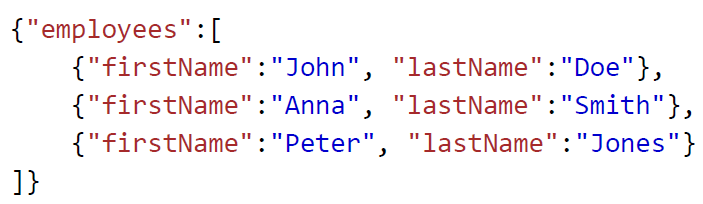
\includegraphics[width=.8\textwidth]{figures/jsonejemplo}
            \end{center}
            \caption{Ejemplo de lista de empleados genérica en \textit{JSON}}
            \label{json-ejemplo}
        \end{figure}
        
        Fue elegido por su compatibilidad con Java y porque es independiente de la tecnología usada en la vista, lo cual permite a su vez realizar cambios en la vista sin afectar las funcionalidades del controlador.
        
        \subsection{JPA}
        \label{tecno-jpa}
        
        Por ``Java Persistence API", proporciona un modelo de persistencia basado en objetos de Java planos (POJO, por sus siglas en inglés \textit{Plain Old Java Object}) para hacer la correspondencia con las entidades en la base de datos\cite{JPA-definicion}. En la práctica, hace transparentes las consultas y acciones realizadas sobre la base de datos.
        
        Como tal, JPA, no implementa los modelos de persistencia que usará la base de datos si no que proporciona un estándar para que se puedan mantener las caractarísticas de la orientación a objetos de Java y se puedan enlazar, uno a uno, con las entidades, atributos y relaciones de la base de datos.
        
        JPA se puede configurar vía anotaciones o usando un documento XML que debe ser distribuido junto con el sistema. En el caso de ``HxPlus Ocupacional" se eligió la configuración por anotaciones debido que está presente directamente en los objetos (clases) de Java y permite una mejor mantinibilidad del código.
        
        Entre las implementaciones conocidas de JPA tenemos:
        \begin{itemize}
             \item Hibernate
             \item ObjectDB
             \item EclipseLink
             \item OpenJPA
        \end{itemize}
        
        Siendo la implementación de Hibernate la seleccionada por lo descrito en el punto \ref{tecno-hibernate}.
        
        \subsection{Angular JS}
        \label{tecno-angular}
        
        Es un \textit{framework} orientado a facilitar el desarrollo web de aplicaciones dinámicas del lado del cilente. ``AngularJS le permite extender el vocabulario HTML para su aplicación"\cite{ANGULARJS-angularjs}. Utiliza lo que llama ``directivas" que son bloques de código en javascript que ayudan a estructurar las acciones del \textit{front-end}. También maneja ``atributos" y ``elementos" que pueden ser programados separadamente del código HTML y luego insertados en dicho archivo para su utilización.
        
        Provee asociación birireccional de variables del DOM lo cual simplifica drásticamente las pruebas del lado del cliente y mantiene, como se mencionó anteriormente, la estructura organizada del código. La asociación bidireccional a través de ``expresiones" se utiliza para mantener actualizado al cliente en cuanto a cambios que se realizen en las variables internas y mejora la respuesta visual sin realizar una recarga de la página.
        
        El código de Javascript (punto \ref{tecno-javascript}) debe ser importado en el archivo HTML en que se quieren utilizar. Existen dos formas de importarlas, desde el servidor de google\footnote{http://ajax.googleapis.com/ajax/libs/angularjs/1.4.8/angular.min.js} o descargando los archivos al servidor local y agregando la dirección local.
        
        Por todo esto, se eligió AngularJS para su utilización como \textit{framework} del \textit{front end} del sistema.
        
        \subsection{JavaScript}
        \label{tecno-javascript}
        
        JavaScript es un lenguaje de programación interpretado, dialecto del estándar ECMAScript. Se define como orientado a objetos, basado en prototipos, imperativo, débilmente tipado y dinámico \cites{JAVASCRIPT-wiki}{JAVASCRIPT-manual}. También posee soporte en casi todos los navegadores utilizados actualmente.
        
        Es un lenguaje de programación orientado a crear contenidos dinámicos para páginas web del lado del cliente. AngularJS, previamente mencionado, usa JavaScript como lenguaje de programación para su implementación.
        
        \subsection{MySQL}
        \label{tecno-mysql}
        
        Gestor de bases de datos, posee licencia GPL y licencia comercial de Oracle\cite{MYSQL-referencemanual}. Ofrece alto rendimiento, eficiencia y seguridad en el almacenamiento y recuperación de datos\cite{MYSQL-oracle}. Comúnmente utilizado en entornos de desarrollo LAMP para desarrollo web.
        
        Es un gestor multi-hilo, multi-usuario y robusto, está diseñado para soportar altos niveles de carga y ser utilizado en entornos de producción con fuerte afluencia de datos. Además de poseer librerías ampliamente usadas para Java las cuales ayudan al desarrollo debilmente acoplado del \textit{back-end}.
        
        Para ``HxPlus Ocupacional" se eligió este gestor, haciendo uso de su licencia GPL, para el desarrollo del sistema.
        
        \subsection{SPRING}
        \label{tecno-spring}
        
        Framework para el desarrollo de aplicaciones que provee inversión de control; es de código abierto y está diseñado sobre Java. Permite integración con Hibernate, JPA y JSON\cite{SPRING-essential}.
        
        SPRING fue diseñado para facilitar el desacoplamiento de los compomentes del sistema utilizando inversión de control. Esto permite que los componentes sean desarrollados una y sólo una vez y que puedan ser reutilizados en diferentes contextos\cite{SPRING-referencedoc}.
        
        Su fácil integración con Hibernate y, por consecuencia, con JPA permite que la interacción con la base de datos sea transparente al desarrollador y evita que tenga que reescribirse el código en caso de cambios en el gestor (de bases de datos) utilizados.
        
        
        \subsection{Maven}
        \label{tecno-maven}
        
        Es una herramienta de gestión y manejo de librerías, parecida a ``Apache Ant". Utiliza el concepto del ``Modelo del Objeto de Proyecto" (del inglés \textit{Project Object Model}, o POM) para gestionar la construcción del proyecto dónde se utilice. Esto es, gestiona las librerías, dependencias y versiones (de las librerías) de forma centralizada y limpia.
        
        El POM es un archivo en formato XML dónde se registran las librerías que serán usadas por el proyecto  para que el gestor de Maven se encargue de la descarga de las mismas. Se gestiona a través de artefactos que registran la información de una librería de acuerdo con la figura \ref{pom-artifact}.
        
        \begin{figure}[htbp!]
            \begin{center}
                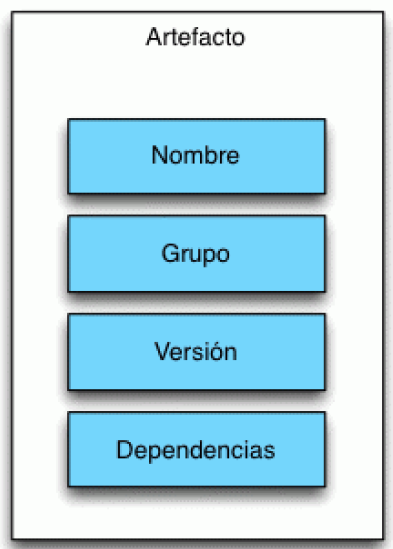
\includegraphics[scale=0.4]{figures/pomartifact}
            \end{center}
            \caption{Artefacto de Maven y descripción de su contenido.}
            \label{pom-artifact}
        \end{figure}
        
        La estructura del POM puede llegar a ser tan compleja como el proyecto que gestiona, llegando incluso a depender de otros POM. En ``HxPlus Ocupacional" se manejó usando un sólo POM de la manera más sencilla posible.
        
        En \citetitle{APACHE-maven}\cite{APACHE-maven} mantienen repositorios de librerías actualizados y correctamente asociados a las dependencias de dichas librerías.
        
        \subsection{Hibernate}
        \label{tecno-hibernate}
        
        Es un framework de persistencia que provee una implementación de JPA\cite{HIBERNATE-basico}. Gestiona las comunicaciones a nivel de nombres de entidades y atributos con su respectiva contraparte de Java, clases con sus atributos. A esto se le conoce como ``Correlación Objeto-Relacional" (ORM, por su siglas en inglés \textit{Object Relational Mapping}).
        
        Esta correlación que crea Hibernate permite ciertas facilidades al momento de manejar las distintas interacciones con la base de datos que devienen en un código mantenible en el tiempo.
        
        El framework es integrado al desarrollo a través de Maven y tiene soporte para los siguientes gestores de bases de datos\cite{HIBERNATE-tutorial}: 
        \begin{itemize}
            \item MySQL
            \item PostgreSQL
            \item Oracle
            \item DB2/NT
            \item HSQL Database Engine
            \item entre otros...
        \end{itemize}
        
        Tradicionalmente se utilizan dos archivos de configuración (llamados ``hibernate.properties" y ``hibernate.cgf.xml") que se modifican con cada nueva tabla o ``clase de persistencia" que se requiera, sin embargo este método tiende a no ser mantenible en el tiempo ya que debe buscarse dentro de estos archivos las configuraciones de las clases y no existe un orden estipulado para la creación y modificación de estos archivos. Para evitar esto, y dado que se tiene una versión de Java opsterior a JDK 5, se procedió a la utilización de la versión 3 de hibernate que incorpora librerías para el uso de anotaciones, quedando así la configuración de las clases de persistencia dentro del código de las clases de Java, lo cual permite y permitió, durante el desarrollo, fácil depuración de errores y un sencillo mantenimiento del código.
        
        \subsection{iText}
        \label{tecno-itext}
        
        Herramienta de generación de PDF dinámicos\cite{ITEXT-basico}. Proporciona un API que permite la generación de archivos PDF usando la información enviada.
        
        Actualmente existen módulos de gestión, interpretación y conversión de archivos PDF, sin embargo para efectos de ``HxPlus Ocupacional" sólo se utilizó el módulo de generación de los mismos.
        
        Su integración con Maven permitió la fácil descarga de la librería y su configuración dentro del proyecto. Para su uso sólo se necesitó la creación de una clase dentro del \textit{back end}, que contiene las importaciones requeridas para así poder generar los PDF necesarios.
        
    \section{Herramientas para el control de versiones y planificación}
    
    En la presente sección se presentan las herramientas de planificación y control de versiones usadas durante el desarrollo de la aplicación. Si bien no están vinculadas directamente al código, las mismas sirvieron de soporte para la organización del proyecto.
    
        \subsection{Git}
        \label{tecno-git}
        
        Es un sistema de control de versiones distribuido, diseñado por Linus Torvalds, enfocado en eficiencia, integridad de datos, velocidad de transferencia y soporte para flujos de trabajo no lineales.
        
        Siguiendo este enfoque, se logró un \textit{software} que almacena los archivos relativos a un proyecto tomando como base un directorio ``raiz" y los archivos y directorios que lo conformen, incluye recursivamente los archivos y directorios dentro del directorio raiz, y  a partir de ellos almacena los cambios realizados a la última versión, sin modificar los archivos originales ni los archivos de modificaciones; con ello se logra que los cambios puedan ser reversibles y que sean almacenados con poco uso de memoria, reduce la carga de datos al momento de crear repositorios remotos ya que no se está enviando los archivos completos sino los archivos de cambios.
        
        Para el caso de repositorios remotos y el manejo de la carga, también incluye la restricción de versiones. Un usuario debe tener en el repositorio local la última versión disponible, en caso de que la última versión esté en el repositorio local, se cargan los cambios normalmente al repositorio remoto; en caso contrario, el usuario debe descargar la última versión del repositorio remoto, (potencialmente) resolver conflictos que puedan surgir entre los archivos modificados de manera local y los que hayan sido modificados en el servidor remoto y luego hacer la carga al servidor remoto.
        
        También ofrece la posibilidad de crear ``ramas" de desarrollo. Esto es, cambios y modificaciones de un proyecto que parten de una raiz pero que puede tener una meta diferente. Esto facilita el proceso cuando existen varios desarrolladores trabajando en paralelo sobre el mismo proyecto, aunque en el caso de surgir conflictos en los cambios puede llegar a ser engorrosa la integración (\textit{merge}) del código.
        
        Para HxPlus se crearon dos repositorios raices, dadas implicaciones de permisos de ejecución dentro del sistema operativo elegido. Estos repositorios fueron llamasdos ``occupational" y ``proyectoAngular" refiriendose al \textit{back-end} y \textit{front-end} respectivamente.
        
        \subsection{GitHub}
        \label{tecno-github}
        
        Servidores online de repositorios remotos para Git. Puede ser usado de manera gratuita y pública. Permite el acceso a los repositorios de manera ininterrumpida y global.
        
        Los repositorios fueron almacenados en la cuenta personal de Alejandro Tarazona, en el url:\\ \textit{http://www.github.com/atarazona89} con los nombres descritos con anterioridad, para su almacenamiento en la web.
        
        \subsection{Trello}
        \label{tecno-trello}
        
        Herramienta diseñada con la misión de facilitar la gestión de tareas usando listas o tablas. Cuenta con una interfaz intuitiva y de fácil aprendizaje para llevar a cabo dicha misión. Una vez creadas las tablas que se desean, se pueden crear tareas dentro de ellas, las cuales a su vez pueden ser etiquetadas, organizadas o comentadas por los participantes. Las tareas pueden ser arrastradas entre las listas emulando así la transición entre los estados de desarrollo del proyecto.
    
\pagebreak